\documentclass[11pt,a4paper]{article}
\usepackage[utf8]{inputenc}
\usepackage[T1]{fontenc}
\usepackage[french]{babel}
\usepackage[a4paper,margin=2.3cm]{geometry}
\usepackage{graphicx}
\usepackage{xcolor}
\usepackage{booktabs}
\usepackage{enumitem}
\usepackage{titlesec}
\usepackage{fancyhdr}
\usepackage{amssymb}
\usepackage[colorlinks=true,linkcolor=problue,urlcolor=problue]{hyperref}

\definecolor{problue}{RGB}{20,80,150}
\definecolor{progray}{RGB}{90,90,90}
\definecolor{prolight}{RGB}{236,242,248}
\definecolor{progreen}{RGB}{30,120,60}

\graphicspath{{./}{./images/}}

\titleformat{\section}{\color{problue}\large\bfseries}{\thesection.}{0.6em}{}
\titleformat{\subsection}{\color{progray}\normalsize\bfseries}{\thesubsection}{0.6em}{}

\pagestyle{fancy}
\fancyhf{}
\lhead{\small\color{progray}ProtoVA 2 — Rapport hebdomadaire}
\rhead{\small\color{progray}Douae Sebti}
\cfoot{\small\color{progray}\thepage}
\renewcommand{\headrulewidth}{0.4pt}

\newcommand{\ok}{\textcolor{progreen}{$\checkmark$}}

\begin{document}

% ---------- En-tête ----------
\begin{center}
{\color{problue}\Large\bfseries Rapport hebdomadaire — Projet ProtoVA 2}\\[4pt]
{\large Remise en route de la Jetson et fiabilisation de la communication V2V}\\[10pt]
\begin{tabular}{rl}
\textbf{Auteure :} & Douae Sebti \\
\textbf{Projet :} & ProtoVA 2 — véhicule autonome à échelle réduite \\
\textbf{Tuteur académique :} & Samuel Dupont \\
\textbf{Semaine :} & du 21 au 24 juillet 2026 \\
\end{tabular}
\end{center}
\vspace{4pt}
\hrule
\vspace{10pt}

% ---------- 1. Contrainte de la semaine ----------
\section{Contrainte majeure de la semaine}
La semaine a été marquée par un \textbf{incident matériel bloquant} : la carte
\textbf{Jetson Orin Nano} du véhicule ne démarrait plus (alimentation présente, mais
plus aucune sortie HDMI, plus de détection des ports USB ni du WiFi). Le système
d'exploitation, installé sur le SSD NVMe, était corrompu.

La contrainte a donc été double : \emph{(i)} remettre la carte en état de marche sans
perdre le travail accumulé, et \emph{(ii)} reconstruire l'intégralité de
l'environnement logiciel (ROS 2, espace de travail, pile V2V) sur un système neuf.
J'ai d'abord confirmé que la carte était toujours vivante au niveau du bootloader
(détection en \emph{mode recovery}), ce qui a permis de la reflasher plutôt que de la
remplacer.

% ---------- 2. Remise en route ----------
\section{Remise en route complète du système}
J'ai reconstruit l'environnement étape par étape. Le tableau ci-dessous récapitule les
modifications et interventions réalisées cette semaine.

\begin{center}
\renewcommand{\arraystretch}{1.25}
\begin{tabular}{@{}p{5.3cm}p{9.2cm}@{}}
\toprule
\textbf{Élément} & \textbf{Intervention} \\
\midrule
Système d'exploitation & Reflash \textbf{JetPack 6.2.1} (Ubuntu 22.04) via le mode recovery et SDK~Manager \\
WiFi & Pilote Intel \texttt{iwlwifi} absent de JetPack~6.2 $\rightarrow$ recompilé via \texttt{backport-iwlwifi-dkms} (WiFi rétabli) \\
ROS 2 & Réinstallation de \textbf{ROS~2 Humble} + dépendances (twist\_mux, slam\_toolbox, navigation2\ldots) \\
Espace de travail & Recompilation de \texttt{protova2\_yass} (16 paquets) \\
Communication V2V & Reconstruction de \textbf{Vanetza / socktap} avec les applications \textbf{CAM} et \textbf{DENM} \\
Dépendances manquantes & Ajout de \texttt{pyserial}, \texttt{tf\_transformations}, règles udev caméra \\
Sauvegarde & Archivage complet du projet sur un dépôt Git privé \\
\bottomrule
\end{tabular}
\end{center}

\subsection{Validation du matériel}
Une fois le système reconstruit, j'ai vérifié chaque capteur~/ actionneur :
\begin{itemize}[leftmargin=1.4em,itemsep=1pt]
  \item \ok~\textbf{Caméra Orbbec Femto Bolt} : flux couleur + profondeur alignée (15~fps).
  \item \ok~\textbf{LiDAR RPLIDAR A1} : identifié comme modèle A1 (débit \textbf{115200}, et non 256000 comme configuré à tort) ; publication du \texttt{/scan} à $\sim$7,4~Hz.
  \item \ok~\textbf{Microcontrôleur Pico (RP2040)} : liaison série rétablie sur \texttt{/dev/ttyACM0}.
\end{itemize}

% ---------- 3. V2V ----------
\section{Communication V2V : validation de bout en bout}
La chaîne V2V a été validée entre les deux véhicules (le PC et la Jetson) : émission,
transmission WiFi, réception et décodage des messages normalisés ETSI C-ITS.

\begin{figure}[h]
\centering
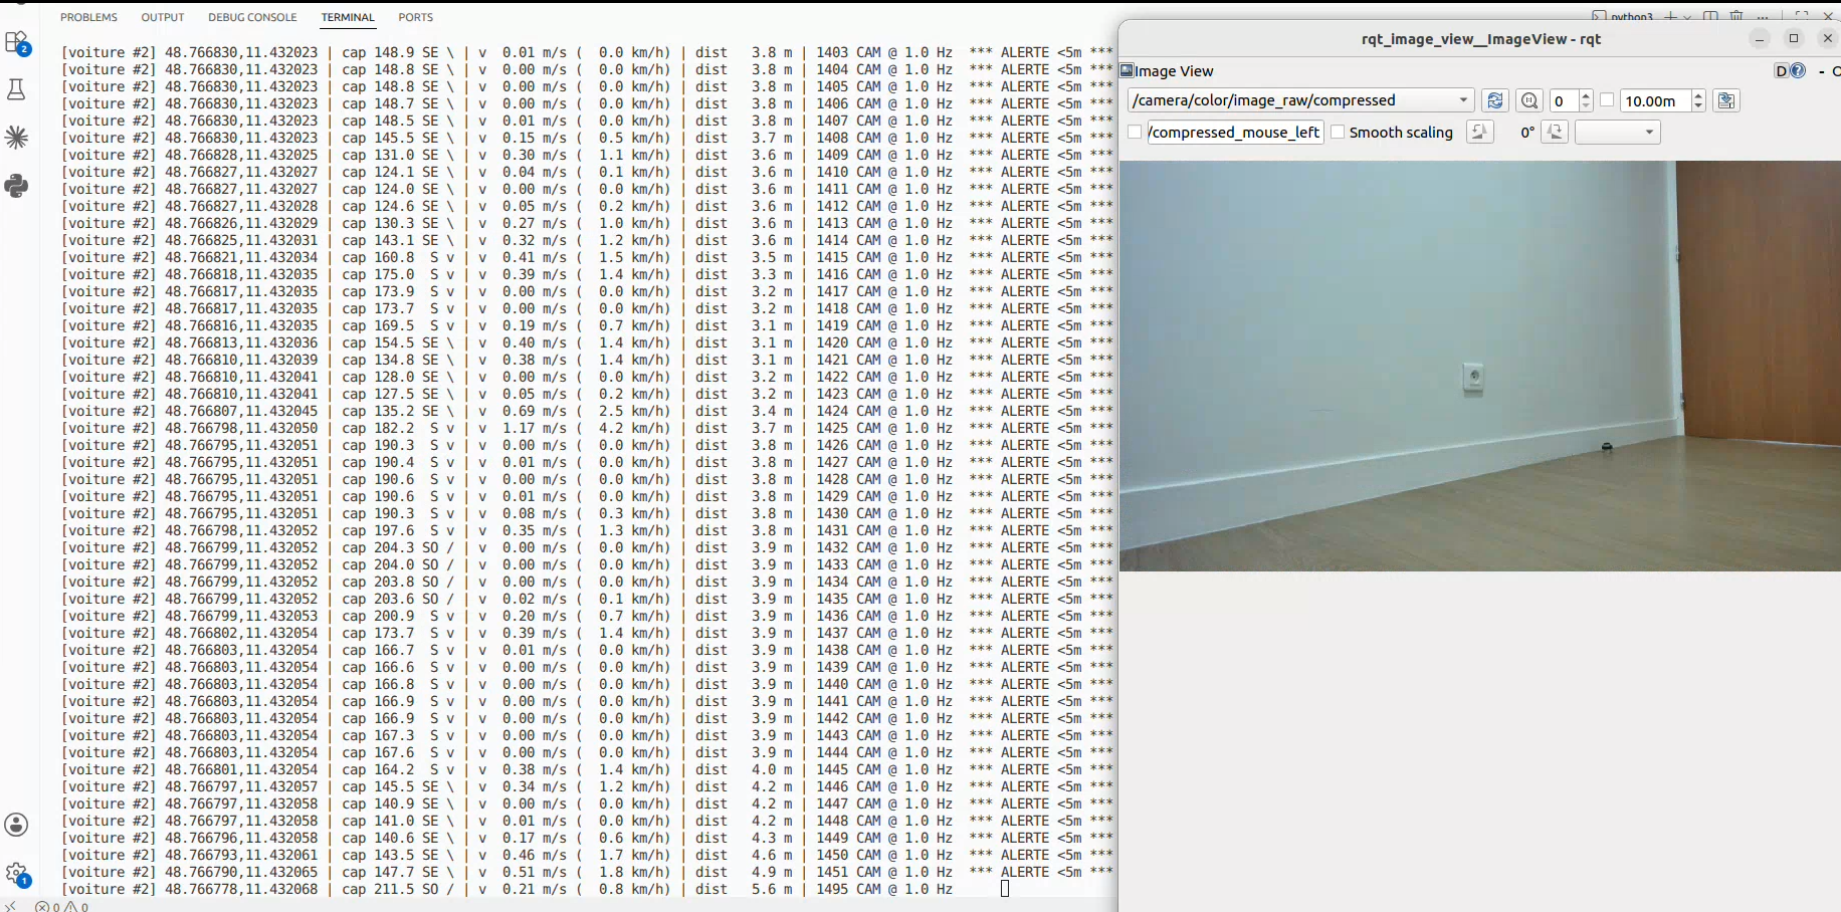
\includegraphics[width=0.82\textwidth]{cam_msg.png}
\caption{Message \textbf{CAM} (position, cap, vitesse) émis et reçu entre les deux véhicules.}
\end{figure}

\begin{figure}[h]
\centering
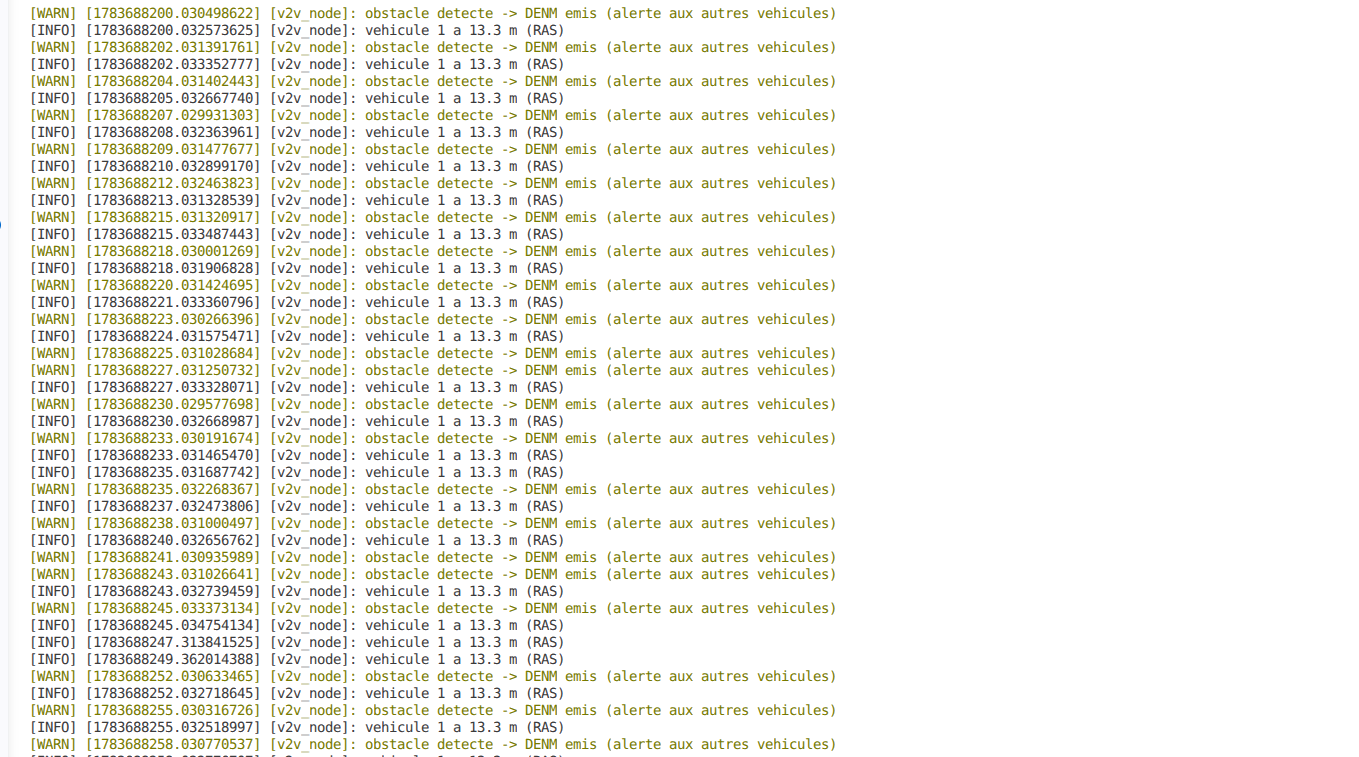
\includegraphics[width=0.82\textwidth]{denm_messages.png}
\caption{Message \textbf{DENM} d'urgence (cause 99 / sous-cause 2 : freinage d'urgence) reçu par le véhicule voisin.}
\end{figure}

% ---------- 4. Problème distance ----------
\section{Problème identifié et résolu : la distance inter-véhicules}
\subsection{Le problème}
La distance affichée entre les deux véhicules était \textbf{erronée et figée}
(p.~ex. « 20,5~m » puis « 8,1~m » alors que les deux appareils n'étaient distants que
de quelques centimètres). Le calcul de distance repose sur les positions géographiques
échangées dans les messages CAM ; or \textbf{aucun véhicule ne possède de GPS}. Les
coordonnées étaient donc \emph{écrites en dur} dans les scripts (points fictifs), et la
distance n'était qu'une constante inventée, insensible aux déplacements.

Un GPS classique n'est pas une solution à cette échelle : son erreur de 2 à 5~mètres est
bien supérieure à la distance à mesurer, et il ne fonctionne pas en intérieur.

\subsection{La solution : mesure par LiDAR}
J'ai exploité le capteur déjà embarqué et le plus précis à cette échelle, le
\textbf{LiDAR}. Un nœud dédié (\texttt{lidar\_neighbor}) extrait du balayage laser la
\textbf{distance réelle} au véhicule voisin (précision centimétrique), et cette mesure
est injectée dans le message V2V. La distance affichée est désormais
\textbf{réelle, dynamique et vérifiable} : elle évolue correctement lorsque le robot ou
le véhicule voisin se déplace.

\begin{center}
\fcolorbox{problue}{prolight}{\parbox{0.93\textwidth}{\ttfamily\small
*** ALERTE V2V *** \ FREINAGE D'URGENCE signalé par le véhicule 2\\
Cause : Situation dangereuse (freinage d'urgence)\\
Distance au véhicule émetteur : \textbf{$\sim$0.36 m} (mesure LiDAR réelle)
}}
\end{center}
\vspace{2pt}
\begin{center}\small\color{progray}
Résultat obtenu en fin de semaine : la distance affichée ($\sim$0,36--0,40~m) correspond
à la distance physique réelle, et varie en temps réel.
\end{center}

% ---------- 5. Perception ----------
\section{Perception et déclenchement de l'alerte}
Le déclenchement de la DENM repose sur la détection caméra (YOLO + profondeur) : la
DENM n'est émise que sur un \textbf{danger confirmé} (piéton, distance $<$~5~m,
persistance sur plusieurs images), ce qui évite les fausses alertes sur le mobilier.

\begin{figure}[h]
\centering
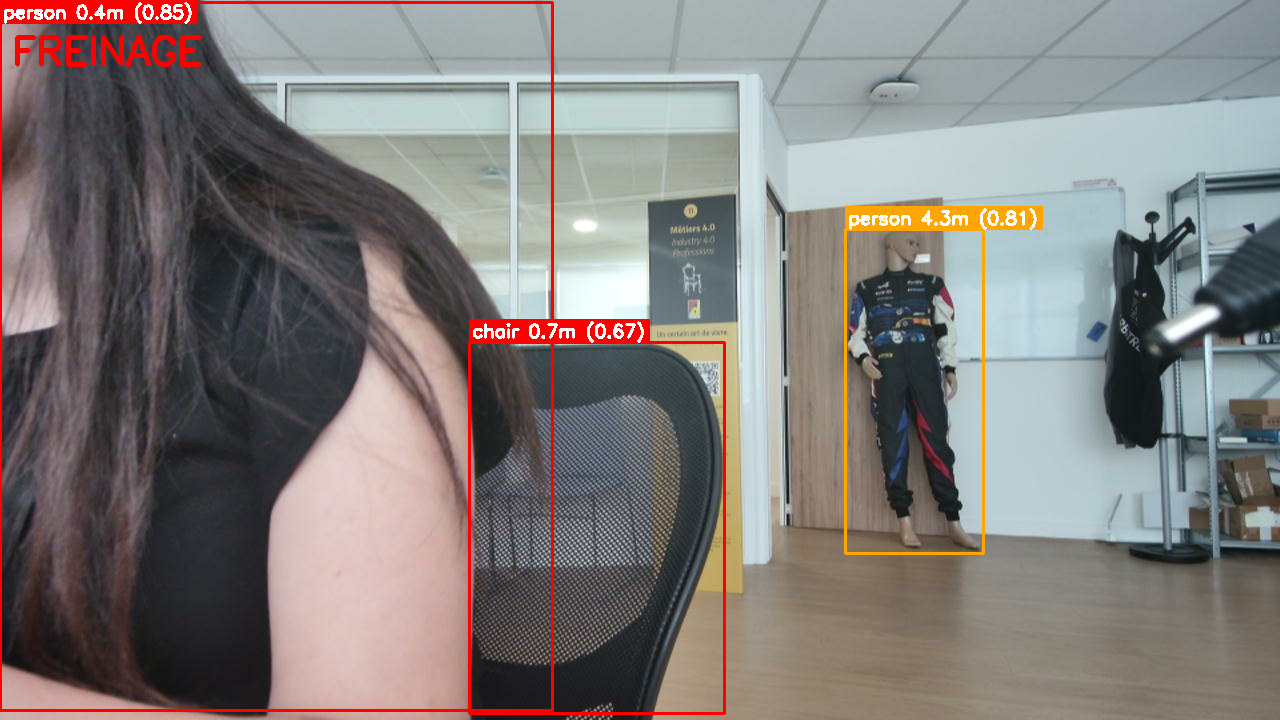
\includegraphics[width=0.72\textwidth]{img_detection_yolo.png}
\caption{Détection YOLO avec distance par profondeur : chaque obstacle est étiqueté (classe + distance).}
\end{figure}

% ---------- 6. Sauvegarde ----------
\section{Sauvegarde et archivage}
Suite à la panne, l'ensemble du projet a été archivé sur un \textbf{dépôt Git privé} :
espace de travail ROS~2, pile V2V (CAM/DENM), perception, freinage d'urgence, démo~5G,
scripts de lancement et documentation. Le travail est désormais protégé contre toute
nouvelle défaillance matérielle.

% ---------- 7. Bilan ----------
\section{Bilan et prochaines étapes}
\textbf{Bilan.} Malgré la panne matérielle, le véhicule est entièrement remis en état,
la communication V2V (CAM + DENM) fonctionne de bout en bout, et le point faible de la
distance fictive a été corrigé par une mesure LiDAR réelle.

\textbf{Prochaines étapes.}
\begin{itemize}[leftmargin=1.4em,itemsep=1pt]
  \item Test des actionneurs (direction + moteur) avec la voiture au sol.
  \item Démonstration terrain complète en mouvement (distance dynamique).
  \item Portage de la détection YOLO sur la Jetson (TensorRT) et essai de la liaison 5G.
\end{itemize}

\end{document}
